\documentclass[10pt]{article}
\usepackage[polish]{babel}
\usepackage[utf8]{inputenc}
\usepackage[T1]{fontenc}
\usepackage{amsmath}
\usepackage{amsfonts}
\usepackage{amssymb}
\usepackage[version=4]{mhchem}
\usepackage{stmaryrd}
\usepackage{graphicx}
\usepackage[export]{adjustbox}
\graphicspath{ {./images/} }

\title{LIGA MATEMATYCZNA im. Zdzisława Matuskiego GRUDZIEŃ 2019 SZKOŁA PODSTAWOWA \\
 klasy IV - VI }

\author{}
\date{}


\begin{document}
\maketitle
\section*{ZADANIE 1.}
Suma cyfr pewnej liczby dwucyfrowej jest równa 7 . Oblicz sumę tej liczby i liczby o przestawionych cyfrach.

\section*{ZADANIE 2.}
Numery pokoi w pewnym hotelu są liczbami trzycyfrowymi, przy czym cyfra setek oznacza numer piętra, na którym znajduje się pokój. Na którym piętrze znajduje się pokój, którego numer jest sześcianem sumy swoich cyfr?

\section*{ZADANIE 3.}
W pudełku jest sześć karteczek, każda biała lub czarna. Na pięciu z nich zapisane są liczby 5, 7, 8, 9, 13 (na każdej kartce jedna liczba). Jaka najmniejsza liczba całkowita dodatnia może być zapisana na szóstej kartce, jeżeli suma liczb z białych kartek jest równa sumie liczb z czarnych kartek?

\section*{ZADANIE 4.}
Herb jednego z matematycznych rodów składa się z nałożonych na siebie dwóch figur: trójkąta równobocznego i pięciokąta foremnego (jak na rysunku). Oblicz miary kątów \(\alpha\) i \(\beta\).\\
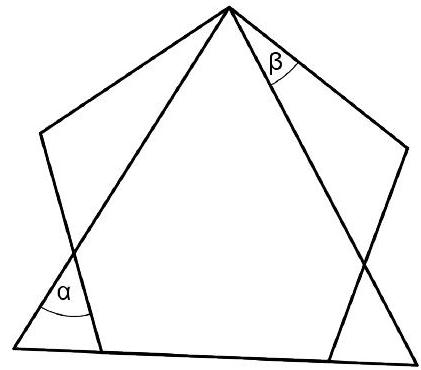
\includegraphics[max width=\textwidth, center]{2024_11_21_57c1852a5ff6e5801ef3g-1(1)}

\section*{ZADANIE 5.}
Prostokąt o obwodzie 42 podzielono na dwa prostokąty i sześć kwadratów tak, jak na rysunku. Oblicz obwód prostokąta \(A\).\\
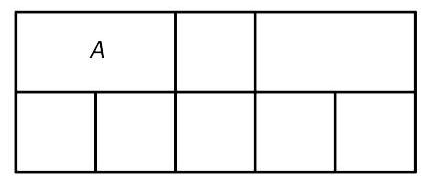
\includegraphics[max width=\textwidth, center]{2024_11_21_57c1852a5ff6e5801ef3g-1}


\end{document}